\documentclass[screen, aspectratio=169]{beamer}
\usepackage[T1]{fontenc}
\usepackage[utf8]{inputenc}
\usepackage{tikz, environ, siunitx, pgfpages}
\usepackage{listings}

\makeatletter
\defbeamertemplate*{note page}{mynotes}
{%
	{%
		\scriptsize
		\usebeamerfont{note title}\usebeamercolor[fg]{note title}%
		\ifbeamercolorempty[bg]{note title}{}{%
			\insertvrule{.45\paperheight}{note title.bg}%
			\vskip-.45\paperheight%
			\nointerlineskip%
		}%
		\vbox{
			\hfill\insertslideintonotes{0.45}\hskip-\Gm@rmargin\hskip0pt%
			\vskip-0.45\paperheight%
			\nointerlineskip
			\begin{pgfpicture}{0cm}{0cm}{0cm}{0cm}
				\begin{pgflowlevelscope}{\pgftransformrotate{90}}
					{\pgftransformshift{\pgfpoint{-2cm}{0.5cm}}%
						\pgftext[base,left]{\usebeamerfont{note date}\usebeamercolor[fg]{note date}\the\year-\ifnum\month<10\relax0\fi\the\month-\ifnum\day<10\relax0\fi\the\day}}
				\end{pgflowlevelscope}
		\end{pgfpicture}}
		\nointerlineskip
		\vbox to .45\paperheight{\vskip0.5em
			\hbox{\insertshorttitle[width=8cm]}%
			\setbox\beamer@tempbox=\hbox{\insertsection}%
			\hbox{\ifdim\wd\beamer@tempbox>1pt{\hskip4pt\raise3pt\hbox{\vrule
						width0.4pt height7pt\vrule width 9pt
						height0.4pt}}\hskip1pt\hbox{\begin{minipage}[t]{7.5cm}\def\breakhere{}\insertsection\end{minipage}}\fi%
			}%
			\setbox\beamer@tempbox=\hbox{\insertsubsection}%
			\hbox{\ifdim\wd\beamer@tempbox>1pt{\hskip8pt\raise3pt\hbox{\vrule
						width0.4pt height7pt\vrule width 9pt
						height0.4pt}}\hskip1pt\hbox{\begin{minipage}[t]{7.5cm}\def\breakhere{}\insertsubsection\end{minipage}}\fi%
			}%
			\setbox\beamer@tempbox=\hbox{\insertshortframetitle}%
			\hbox{\ifdim\wd\beamer@tempbox>1pt{\hskip12pt\raise3pt\hbox{\vrule
						width0.4pt height7pt\vrule width 9pt
						height0.4pt}}\hskip1pt\hbox{\insertshortframetitle[width=4cm]}\fi%
			}%
			\vfil}%
	}%
	\ifbeamercolorempty[bg]{note page}{}{%
		\nointerlineskip%
		\insertvrule{.55\paperheight}{note page.bg}%
		\vskip-.55\paperheight%
	}%
	\vskip.25em
	\nointerlineskip
	\insertnote
}
\makeatother

% Use this for having comments for slides ("presenter view"). Requires a pdf-viewer that handles beamer notes, e.g. PDFPC (https://pdfpc.github.io/)
\setbeameroption{show notes on second screen=right}
\setbeamertemplate{note page}[mynotes]

% Use the NTNU-temaet for beamer 
% \usetheme[style=ntnu|simple|vertical|horizontal, 
%     language=bm|nn|en, 
%     smalltitle, 
%     city=all|trondheim|alesund|gjovik]{ntnu2017}
\usetheme[style=horizontal,language=bm]{ntnu2017}

\usepackage[norsk]{babel}

\title[Short title]{Øvingsforelesning 1 Python (TDT4110/TDT4127)}
\subtitle{Introduksjon, Kalkulasjoner}
\author[O.M. Pedersen]{Ole-Magnus Pedersen}
\institute[NTNU]{}
\date{}
%\date{} % To have an empty date


\NewEnviron{transparent}{
	\tikz\node[opacity=0.2,align=left,inner xsep=0]{\parbox[t]{\linewidth}{
			\BODY
		}};
	}

\lstset{language=Python}
\RequirePackage{listings, color, textcomp}
\lstset{
	tabsize=2,
	rulecolor=,
	basicstyle=\ttfamily\small,
	upquote=true,
	aboveskip={1.5\baselineskip},
	columns=fixed,
	showstringspaces=false,
	extendedchars=true,
	literate={æ}{{\ae}}1
			 {ø}{{{\o}}}1
			 {å}{{\aa}}1
			 {Æ}{{\AE}}1
			 {Ø}{{\O}}1
			 {Å}{{\AA}}1,
	breaklines=true,
	breakatwhitespace=true,
	escapeinside={(*}{*)},
	showtabs=false,
	showspaces=false,
	keepspaces=true,
	showstringspaces=false,
	frame=l,
	identifierstyle=\ttfamily,
	keywordstyle=\color[rgb]{1.0,0,0},
	keywordstyle=[1]\color[rgb]{0,0,0.75},
	%keywordstyle=[2]\color[rgb]{0.5,0.0,0.0},
	keywordstyle=[3]\color[rgb]{0.127,0.427,0.514},
	keywordstyle=[4]\color[rgb]{0.4,0.4,0.4},
	commentstyle=\color[rgb]{0.133,0.545,0.133},
	stringstyle=\color[rgb]{0.639,0.082,0.082},
	mathescape
}


\begin{document}

\begin{frame}
  \titlepage
\end{frame}

% Alternatively, special title page command to get a different background
% \ntnutitlepage

\begin{frame}
  \frametitle{Litt om meg}
  \begin{itemize}
  	\item Ole-Magnus Pedersen
  	\item  5. klasse datateknologi
  	\item Vitass i TDT4110
  \end{itemize}
\end{frame}

\begin{frame}
	\frametitle{Oversikt}
	\begin{itemize}
		\item Praktisk info
		\begin{transparent}
			\item Om øvingsforelesningene
			\item Programmering
		\end{transparent}
	\end{itemize}
\end{frame}

\begin{frame}
	\frametitle{Øvingsopplegget}
	\begin{itemize}
		\item Gruppeveiledning og drop-in på sal:
		\begin{itemize}
		    \item Gruppeveiledning har faste tidspunkter, og mulighet for å få mer dyptgående hjelp
		    \item Drop-in for enklere spørsmål/godkjenning av øvinger
		\end{itemize}
		\item 8 av 10 øvinger må bli godkjent, inkludert minst en auditorieøving
	\end{itemize}
\end{frame}

\begin{frame}
	\frametitle{Øvingsopplegget}
	\begin{itemize}
		% \item Tilgjengelige datamaskiner med Python på datasal
		\item Gjøres på egen datamaskin
		\begin{itemize}
			\item Spør Orakeltjenesten om hjelp med installasjon dersom du har problemer
		\end{itemize}
		\item Øvingene leveres på Blackboard
		\begin{itemize}
			\item Må godkjennes på sal av studass innen innleveringsfristen
		\end{itemize}
		\item Studass vil gi dere veiledning
		\item Piazza kan brukes til spørsmål
	\end{itemize}
\end{frame}

\begin{frame}
	\frametitle{Øvingsrom}
	\begin{itemize}
	    \item I Realfagsbygget:
	    \begin{itemize}
	        \item A2-121
    	    \item A2-127
    	    \item A3-103
	    \end{itemize}
	    \vspace{2em}
	    \item Sjekk veiledningsplanen på wiki for å finne ut hvilke rom som er bemannet når
	\end{itemize}
\end{frame}

\begin{frame}
	\frametitle{Oversikt}
	\begin{itemize}
		\begin{transparent}
			\item Praktisk info
		\end{transparent}
		\item Om øvingsforelesningene
		\begin{transparent}
			\item Programmering
		\end{transparent}
	\end{itemize}
\end{frame}

\begin{frame}
	\frametitle{Tidspunkt}
	\begin{itemize}
		\item Onsdag 16:15-18:00 i EL5
		\item Fredag 14:15-16:00 i F1
		\item Fredag 16:15-18:00 i R1
		\item Forskjellige paralleller har samme pensum hver uke
		\item Info finnes på Blackboard og itgk.idi.ntnu.no
	\end{itemize}
\end{frame}

\begin{frame}
	\frametitle{Timing}
	\begin{itemize}
		\item Vi prøver å få til at teori introduseres i forelesninger før det blir tatt opp her
		\item Hovedsakelig repetisjon og trening fra forrige ukes programmeringsforelesninger
		\begin{itemize}
		    \item Forberedelse for øvinger
		\end{itemize}
		\item Gi beskjed om det blir for liten tid mellom øvingsforelesninger og innleveringsfrist
	\end{itemize}
\end{frame}

\begin{frame}
	\frametitle{Målgruppe for øvingsforelesningene}
	\begin{itemize}
		\item De som ikke synes det er kjempelett
		\begin{itemize}
			\item Unngår dypdykk utenfor pensum
			\item Dersom det trengs mer tid på noe grunnleggende prioriteres det over nytt stoff
		\end{itemize}
		\item Vanskeligere spørsmål mottas, men det er mulig de blir besvart etter timen eller i pausen
	\end{itemize}
\end{frame}

\begin{frame}
	\frametitle{Innhold i øvingforelesningene}
	\begin{itemize}
		\item Gå gjennom løsning på forrige øving
		\begin{itemize}
			\item Avhengig av deres ønsker
		\end{itemize}
		\item Gå gjennom oppgaver som ligner på de gitt i neste øving
		\item Lite teori
		\item Fokus på programmering
		\begin{itemize}
			\item Ta med egen PC (med fullt batteri)!
		\end{itemize}
	\end{itemize}
\end{frame}

\begin{frame}
	\frametitle{Tanken bak innholdet}
	\begin{itemize}
		\item Teori kan man lese i boka
		\item Programmering må man øve på
		\begin{itemize}
			\item Øvelse gjør mester!
			\item Alle kan lære dette
		\end{itemize}
		\item Dersom gjennomgang av teori er ønskelig kan vi gjøre det også
		\begin{itemize}
			\item Kom med innspill, timene er til for deres hjelp
		\end{itemize}
	\end{itemize}
\end{frame}

\begin{frame}
	\frametitle{Øvelse}
	\begin{itemize}
		\item Kan ikke sies for ofte, jo mer du prøver jo mer lærer du
		\item Det er veldig lett å prøve med Python!
		\begin{itemize}
			\item Det verste som kan skje er at programmet ikke fungerer
		\end{itemize}
	\end{itemize}
\end{frame}

\begin{frame}
	\frametitle{Studentassistener/\allowbreak Læringsassistenter (aka. studass)}
	\begin{itemize}
		\item Studass er ikke bare på sal for å godkjenne
		\item Planlegg gjerne å jobbe med øvingen på sal til saltider (gruppeveiledning)
		\item Det er mer travelt de siste timene før fristen
		\begin{itemize}
			\item Bør være klar for innlevering på dette tidspunktet
		\end{itemize}
	\end{itemize}
\end{frame}

\begin{frame}
	\frametitle{Mentalitet}
	\begin{columns}
		\begin{column}{.4\textwidth}
			\begin{itemize}
				\item Programmering handler om problemløsning
				\item Vi løser oppgaver vha. programmering.
			\end{itemize}
		\end{column}
		\hfill
		\begin{column}{.4\textwidth}
			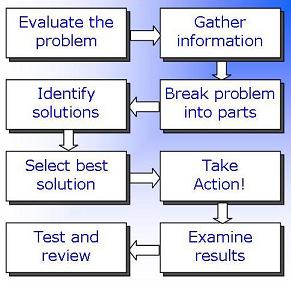
\includegraphics[width=\textwidth]{programmering}
		\end{column}
	\end{columns}
\end{frame}

\begin{frame}
	\frametitle{Oversikt}
	\begin{itemize}
		\begin{transparent}
			\item Praktisk info
			\item Om øvingsforelesningene
		\end{transparent}
		\item Programmering
	\end{itemize}
\end{frame}

\begin{frame}{Hvordan kjøre Python?}
\begin{itemize}
	\item Kjøre en og en kommando:
	\begin{itemize}
		\item Interactive mode
		\item Idle eller terminal/kommandolinje
	\end{itemize}
	\item Skrive lengre filer med programmer og kjøre dem
	\begin{itemize}
		\item Måten som brukes til vanlig (bl.a. fordi man da kan lagre programmene sine)
		\item Idle
		\item Vanlig teksteditor og terminal/kommandolinje
		\item PyCharm
	\end{itemize}
\end{itemize}
\end{frame}

\begin{frame}{Pycharm Editor}
	\begin{itemize}
		\item \href{https://www.jetbrains.com/pycharm/}{https://www.jetbrains.com/pycharm/}
		\item Mer stabilt enn IDLE på noen OS
		\item Lettere å bruke når man blir vant til det
	\end{itemize}
\end{frame}

\begin{frame}[fragile]{Setup av PyCharm}
	\begin{enumerate}
		\item Lag et nytt prosjekt og gi det et navn
		\item Lag en ny python fil for å begynne å programmere
		\item Skriv et program som printer "æ ø å Æ Ø Å"
		\begin{itemize}
			\item \lstinline|print("æ ø å Æ Ø Å")|
		\end{itemize}
	\end{enumerate}
\end{frame}

\begin{frame}[fragile]{Setup av Pycharm}
	\begin{itemize}
		\item Dersom programmet krasjer må du endre noe
		\item Gå til file $\rightarrow$ settings $\rightarrow$ editor $\rightarrow$ file encodings
		\item Sett IDE og PROJECT ENCODING til UTF-8
		\item Prøv å kjør programmet igjen
		\item Dersom du får feil igjen, kjør programmet med (øverst):
		\begin{itemize}
			\item \lstinline|# -*- coding: utf-8 -*-|
		\end{itemize}
		\item Dersom det fortsatt ikke fungerer må du unngå norske bokstaver
	\end{itemize}
\end{frame}

\begin{frame}{Python syntaks}
	\begin{itemize}
		\item \emph{Syntaks} er læren om hvordan ord settes sammen til større enheter
		\item Man må vite hvilke verktøy som finnes når en skal løse et problem
		\item Vi starter med enkle ''ord'', mer og mer vil bli introdusert i programmeringsforelesninger
	\end{itemize}
\end{frame}

\note[itemize]{
	\item Vi starter i dag med enkle "ord"
	\begin{itemize}
		\item Matte
		\item Kommentarer
		\item Variabler
		\item Innebygde funksjoner
	\end{itemize}
	}

\begin{frame}[fragile]{Operatorer}
	\begin{itemize}
		\item \lstinline|+, -, *, /|
		\item \lstinline|>, <, ==, %, //, **|
	\end{itemize}
	\begin{itemize}
		\item \lstinline|2 * 4 = 8|
		\item \lstinline|9 + 7 - 4 / 2 = 14|
		\item \lstinline|2 * 6 / 4 = 3|
		\item \lstinline|2 ** 8 = 256|
	\end{itemize}
\end{frame}

\begin{frame}[fragile]{Presedens}
	\begin{columns}
		\begin{column}{.5\textwidth}
			\begin{itemize}
				\item Hvilken rekkefølge utføres operatorer i?
				\item Hva regnes ut først?
				\begin{itemize}
					\only<-1>{
						\item \lstinline|4 + 3 * 2 = ?|
						\item \lstinline|(4 + 3) * 2 = ?|
						\item \lstinline|4 - 6 / 3 - 2 = ?|
						\item \lstinline|(4 - 6) / (3 - 2) = ?|
						\item \lstinline|4 * (2 / 4) = ?|
						\item \lstinline|5 * - 3 = ?|
					}
					\only<2->{
						\item \lstinline|4 + 3 * 2 = 10|
						\item \lstinline|(4 + 3) * 2 = 14|
						\item \lstinline|4 - 6 / 3 - 2 = 0|
						\item \lstinline|(4 - 6) / (3 - 2) = -2|
						\item \lstinline|4 * (2 / 4) = 2|
						\item \lstinline|5 * - 3 = -15|
					}
				\end{itemize}
			\end{itemize}
		\end{column}
		\begin{column}{.4\textwidth}
			\footnotesize
			\begin{block}{\small Presedens og parantesbruk}
				\begin{enumerate}
				    \item \lstinline|**| \hfill eksponensiering
					\item \lstinline|-| \hfill negasjon
					\item \lstinline|* / // %| \hfill multiplikasjon, divisjon, \\\hfill heltallsdivisjon, modulo
					\item \lstinline|+ -| \hfill addisjon, subtraksjon
				\end{enumerate}
				\begin{itemize}
					\item Fra venstre mot høyre
					\item Innenfra og ut
				\end{itemize}
			\end{block}
		\end{column}
	\end{columns}
\end{frame}

\begin{frame}{Oppgaver}
	\begin{itemize}
		\item Start opp Python
		\vspace{1em}
		\item Hva tilsvarer 80 grader celsius i farenheit?
		\begin{itemize}
			\item $F = \frac{9}{5} \cdot Celsius + 32$
		\end{itemize}
	\end{itemize}
\end{frame}

\begin{frame}[fragile]{Oppgave}
	\begin{itemize}
		\item Hva blir \lstinline|7! / (5! - 3)|?
		\begin{itemize}
			\item $7! = 7*6*5*4*2*1$
		\end{itemize}
	\end{itemize}
\end{frame}

\begin{frame}{Oppgave}
	\begin{itemize}
		\item Er \num{1000000000} et større tall enn $2^{30}$?
	\end{itemize}
\end{frame}

\begin{frame}[fragile]{Negasjon}
	\begin{itemize}
		\item Regn ut:
		\only<1>{
			\begin{enumerate}
				\item $4 * -2 - (2 + -5)$
				\item $-2 - -2 - 2$
				\item $5 - 2^{-1*-1}$
				\item $-(1*1*2*3*5*-8)$
			\end{enumerate}
			}
		\only<2>{
			\begin{enumerate}
				\item $4 * -2 - (2 + -5) = -5$
				\item $-2 - -2 - 2 = -2$
				\item $5 - 2^{-1*-1} = 3$
				\item $-(1*1*2*3*5*-8) = 240$
			\end{enumerate}
			}
	\end{itemize}
\end{frame}

\begin{frame}[fragile]{Variabler}
	\begin{itemize}
		\item En variabel er en navngitt plass i minnet, hvor man kan lagre en verdi
		\item Kan slå opp verdien ved å skrive navnet
		\item Kan senere endre verdien
		\item Parallell til matte
	\end{itemize}
	
	\begin{columns}
		\begin{column}{.3\textwidth}
			\begin{gather*}
				x = 123\\
				y = 2^x
			\end{gather*}
		\end{column}
		\begin{column}{.7\textwidth}
			\begin{lstlisting}
x = 123
y = 2 ** x
			\end{lstlisting}
		\end{column}
	\end{columns}
	
\end{frame}

\begin{frame}[fragile]{Løs oppgave vha. en variabel}
	\begin{columns}
		\begin{column}{.5\textwidth}
			\begin{itemize}
				\item Regn ut volumet av en kjegle
				\begin{itemize}
					\item $V=\pi r^2\frac{h}{3}$
				\end{itemize}
				\item Hint: Lagre en variabel \emph{pi} med verdi $3.14$
				\item Oppgave: Regn ut volumet for en kjegle med radius = 3 og høyde = 7
			\end{itemize}
		\end{column}
	\hspace{-20pt}\vrule\hspace{20pt}
		\begin{column}{.4\textwidth}
			{\large\bfseries Ekstra}
			\begin{itemize}
				\item Utvid programmet til å bruke to ekstra variabler, en for radius og en for høyde
				\item Regn ut volumet for kjegle med:
				\begin{enumerate}
					\item $r=3, h=7$
					\item $r=1, h=8$
					\item $r=3, h=2$
				\end{enumerate}
			\end{itemize}
		\end{column}
	\end{columns}
\end{frame}


\begin{frame}[fragile]{Variabeltyper}
	\begin{itemize}
		\item Variabler har en \emph{type} som bestemmer hva slags data de peker på
	\end{itemize}
	\begin{description}
		\item[Integer] Heltallsverdi (eks. 1, 23, -42)
		\item[Float] Desimaltall (eks. 1.0, 33.12, \lstinline|math.pi|)
		\item[Boolean] Kan ha nøyaktig to verdier, \lstinline|True| og \lstinline|False|
		\item[String] Tekst (Eks. \lstinline|"Dette er en streng"|, \lstinline|'Dette er en tekststreng med enkeltfnutter'|)
	\end{description}
	\begin{itemize}
		\item I Python trenger du ikke å si hva slags type en variabel er på forhånd, men det er viktig å være obs på det når man bruker variabelen
	\end{itemize}
\end{frame}

\note{
	Vis et eksempel:\\
	a = "2"\\
	b = 2\\
	c = 3\\
	print(a + c)\\
	print(b + c)\\
	a = 2\\
	b = 2.0\\
	c = 1\\
	print(c/a)\\
	print(c/b)
}

\begin{frame}[fragile]{Konvertere til forskjellige typer}
	\begin{itemize}
		\item Noen ganger har vi en variabel av en type (f.eks. \lstinline|float|), men ønsker verdien i en annen type (f.eks. \lstinline|int|)
		\item Spesielle funksjoner for å ''caste'' variabler til en annen type:
		\begin{itemize}
			\item \lstinline|int(x)|
			\item \lstinline|float(x)|
			\item \lstinline|str(x)|
			\item \lstinline|bool(x)|
		\end{itemize}
		\item Må passe på når de brukes
		\begin{itemize}
			\item Ikke alt kan konverteres til alt: \lstinline|int("Dette er en streng")|
			\item \lstinline|bool("False") = True|
			\item \lstinline|int(23.9) = 23|
		\end{itemize}
	\end{itemize}
\end{frame}

\note[itemize]{
	\item Merk at bool(x) bare er False hvis x er 0 eller tom streng, ellers True
}

\begin{frame}[fragile]{Kommentarer}
	\begin{itemize}
		\item Brukes for å forklare koden, har ingen effekt på programmet
		\item To typer i Python:
		\begin{itemize}
			\item Linjekommentarer merkes med \lstinline|#|
			\begin{itemize}
				\item \lstinline|print("Dette er ikke en kommentar") # Men dette er en|
			\end{itemize}
			\item Blokkkommentarer brukes for å kommentere ut flere linjer, merkes med \lstinline|'''| eller \lstinline|"""| før og etter
		\end{itemize}
	\end{itemize}
	\begin{lstlisting}
"""
Dette er en kommentar
Den går over flere linjer,
helt til man stopper den
"""
print("Dette er ikke en kommentar")
	\end{lstlisting}
\end{frame}

\begin{frame}[fragile]{Innebygde funksjoner}
	\begin{itemize}
		\item \lstinline|round()|
		\item \lstinline|abs()|
		\item \lstinline|min()|
		\item \lstinline|input()|
		\item \lstinline|print()|
		\vspace{1em}
		\item Mer om funksjoner senere i pensum
	\end{itemize}
\end{frame}

\begin{frame}[fragile]{Input}
	\begin{itemize}
		\item Funksjon for å få inn data fra brukeren:
		\begin{itemize}
			\item \lstinline|input("Hva heter du? ")|
			\item Gir alltid en streng tilbake
		\end{itemize}
		\item Lag et program som spør om hvem som har laget det
		\item Lagre inputten i en variabel
		\item Print så: <Lagret navn> har laget dette programmet
		\vspace{1em}
		\item Hint: \lstinline|print(f"Tekst {variabel1} mer tekst {variabel2} ...")|
		\begin{itemize}
			\item For eldre versjoner av Python:
			\begin{itemize}
				\item  \lstinline|print("Tekst", variabel1, "mer tekst", variabel2, "...")|
				\item \lstinline|print("Tekst " + variabel1 + " mer tekst " + variabel2 + " ...")| (Hvis variablene er strenger)
			\end{itemize}
		\end{itemize}
	\end{itemize}
\end{frame}

\begin{frame}{Mer input}
	\begin{itemize}
		\item Lag et program som tar inn to tall fra bruker, multipliserer dem og skriver ut <tall 1> * <tall 2> = <resultat>
	\end{itemize}
\end{frame}

\begin{frame}{Kjegle igjen}
	\begin{itemize}
		\item Endre kjegleprogrammet fra i stad til å ta inn radius og høyde fra brukeren
		\item Verdiene skal være av typen float
	\end{itemize}
\end{frame}

\begin{frame}[fragile]{Innebygde funksjoner}
	\begin{itemize}
		\item Skriv et program som spør om to tall og printer absoluttverdien av differansen
		\item Hint: Bruk den innebygde funksjonen \lstinline|abs()|
	\end{itemize}
\end{frame}

\begin{frame}[fragile]{Importering av moduler}
	\begin{itemize}
		\item Moduler inneholder bl.a. funksjoner som ikke er lastet inn av seg selv
		\item Vi importerer modulene for å ta i bruk funksjonaliteten
		\vspace{1em}
		\only<2>{
			\item Skriv et program som printer Pi med 10 desimaler
			\item Hint: \lstinline|import math, math.pi, round()|
		}
	\end{itemize}
\end{frame}

\begin{frame}[fragile]{Kahoot!}
	\begin{itemize}
		\item \href{https://play.kahoot.it/#/k/f3efe5c8-705e-4a0e-bad0-3d4ca0fd40aa}{Kahoot}
	\end{itemize}
\end{frame}

\begin{frame}{Spørsmål?}
	\begin{itemize}
		\item Send meg eventuelt spørsmål på \href{mailto::olemagnp@stud.ntnu.no}{olemagnp@stud.ntnu.no}
	\end{itemize}
\end{frame}

\end{document}